\documentclass{beamer}

\usepackage{beamerthemesplit} % new
\usepackage[utf8]{inputenc}
\usepackage[spanish,activeacute]{babel}
\usepackage{graphicx}
\graphicspath { {media/} }
\newcommand\floor[1]{\lfloor#1\rfloor}
\newcommand{\Mod}[1]{\ (\mathrm{mod}\ #1)}

%\hypersetup{pdfpagemode=FullScreen}
\begin{document}
\title{AS combinadas \\ Intercambio de llaves \\ Suites criptográficas}   
\author{González Vargas \\ Acosta Hernández} 
\date{Criptografía y seguridad 2017-2 \\ Facultad de Ciencias UNAM} 

\frame{\titlepage} 
\frame{\frametitle{Contenido}\tableofcontents} 


\section{Combinación de Asociaciones de Seguridad}
\subsection{Preliminares}
\frame{\frametitle{Recordando...}
  \begin{itemize}
  \item Asociaciones de seguridad 
  \item Modos de uso en SA
  \end{itemize}
}
\subsubsection{Asociaciones de seguridad}
\frame{\frametitle{Definición}
  Es una conexión lógica de un sólo sentido entre un emisor
  y un receptor que proporciona servicios de seguridad al tráfico de información
  que se transporta en ella.
}

\subsubsection{Modos de uso en SA}
\frame{\frametitle{Modo de transporte}
  \begin{itemize}
  \item Utilizado para cifrar y opcionalmente autentificar los datos de IP.
  \item Adecuado para proteger conexiones entre \textit{hosts}, que soportan \textit{ESP}.\\

    Ventaja: Provee confidencialidad para cualquier aplicación que la utilice.\\
    Desventaja: Es susceptible a análisis de tráfico.
  \end{itemize}
}

\frame{\frametitle{Modo túnel}
  \begin{itemize}
  \item Es utilizado cifrar un paquete IP por completo.
  \item Orientado para sistemas que incluyen un \textit{firewall}, o algún otro
    mecanismo de seguridad que protege una red confiable de redes externas.
    Ventaja: Resistente a análisis de tráfico.
  \end{itemize}
}

\subsection{Combinación de SAs}
\frame{\frametitle{¿Para qué?}
  Una asociación de seguridad puede implementar ya sea un protocolo \textit{AH}
  o un \textit{ESP}, pero sólo uno.
  Sin embargo, puede ocurrir que un flujo de tráfico llame servicios de ambos protocolos
  durante su operación. En otro caso, puede que dicho flujo necesite de los servicios de \textit{IPsec} entre \textit{hosts} y, para ese mismo flujo, servicios separados entre \textit{gateways}.
  Múltiples SAs, deben ser utilizados para obtener los servicios de \textit{IPsec}.
}

\frame{\frametitle{Colecciones de SAs}
  Secuencia de \textbf{SA}s a través de las cuáles el tráfico de datos debe ser procesado
  para obtener los servicios de \textit{IPsec} que se necesitan.
  Se puede obtener una combinación de SAs mediante:
  \begin{itemize}
  \item Transport Adjacency
  \item Iterated Tunneling
  \end{itemize}
}

\frame{\frametitle{Transport Adjacency}
  Consiste en aplicar más de un protocolo de seguridad a un mismo paquete \textit{IP} sin invocar
  un modo túnel. Se realiza sólo un nivel de anidamiento, pues el procesamiento es realzado
  para una única instancia de \textit{IPsec}, el punto de destino del paquete.
}
\frame{\frametitle{Iterated Tunneling}
  Consiste en aplciar múltiples capas de protocolos de seguridad a un paquete, efectuadas a través de tunelizado de \textit{IP}.
  Este enfoque permite varios niveles de anidamiento dado que cada túnel puede originarse o terminar en un punto
  de \textit{IPsec} a lo largo de la trayectoria del paquete.
}

\frame{\frametitle{Combinación}
  Ambos enfoques pueden ser combinados al hacer que, por ejemplo, una \textbf{SA} de transporte entre \textit{hosts} viaje parte del camino por medio de un \textbf{SA} de túnel entre \textit{gateways} de
  seguridad.
  Un interrogante potencial al tener colecciones de \textbf{SA}s, es el orden en que la autentificación y el cifrado deben ser aplicados entre dos puntos de destino y las maneras para conseguir el apropiado.  
}

%i y ii
\subsection{Autentificación y confidencialidad}
\frame{\frametitle{Autentificación y confidencialidad}
  Siempre que la comunicación entre \textit{hosts} requiera tanto de un cifrado como una autentificación, ambos pueden combinarse y aplicarse en la transmisión de paquetes \textit{IP}. 
}

\subsubsection{Diferentes opciones}
\frame{\frametitle{ESP con Autentificación}
  El usuario apica primero \textit{ESP} a la información que debe ser protegida y posteriormente agrega al final el campo de autentificación.  \\
  \vspace{0.3cm}
  Se tienen dos casos:\\
}

\frame{\frametitle{ESP con Autentificación}
  \begin{itemize}
  \item \textbf{Transport Mode ESP}
     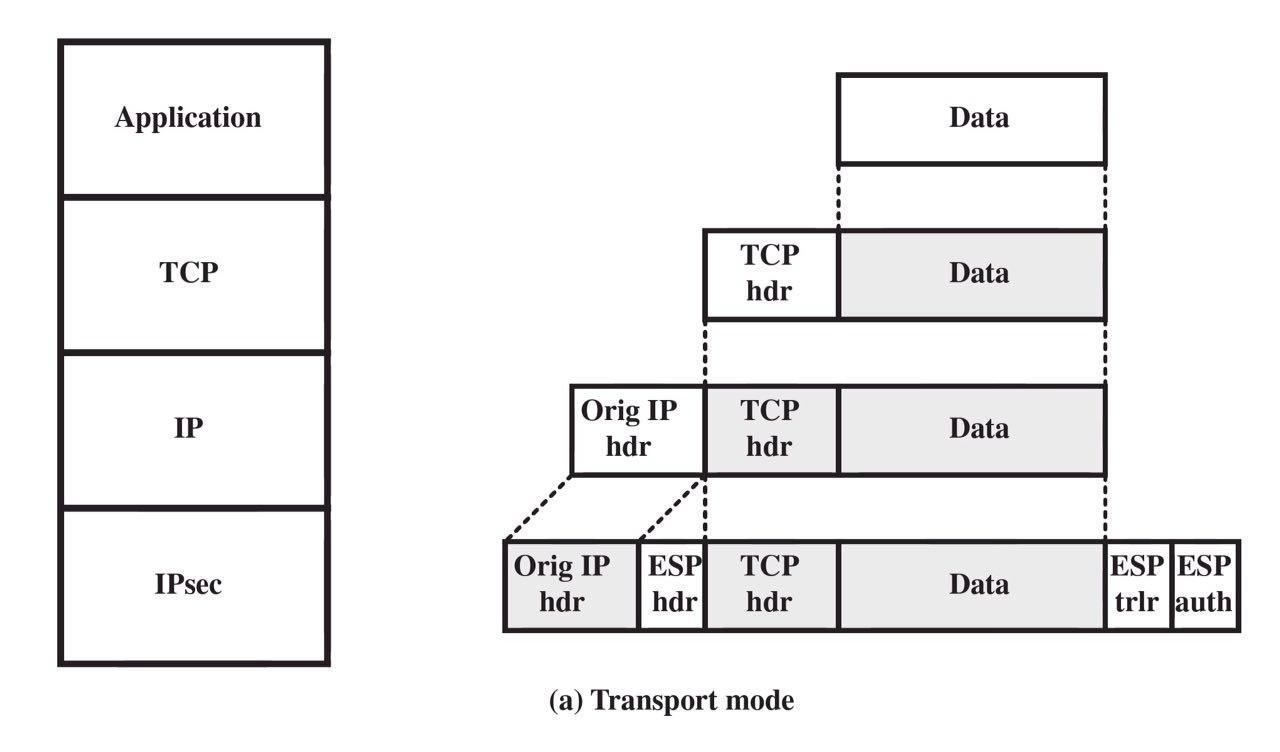
\includegraphics[scale=0.20]{ESPauthTrans.jpg}
    %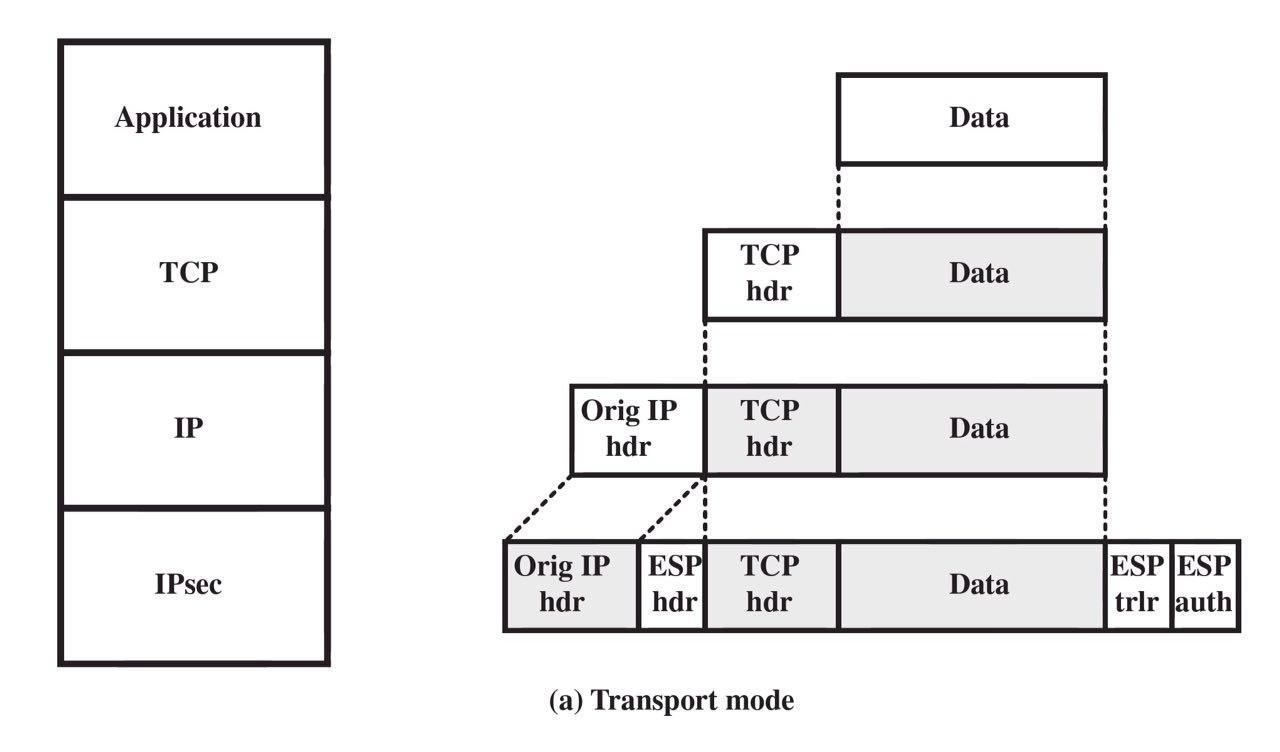
\includegraphics[width=1\textwidth]{ESPauthTrans}
  \end{itemize}
}

\frame{\frametitle{ESP con Autentificación}
  \begin{itemize}
  \item \textbf{Tunnel Mode ESP}
    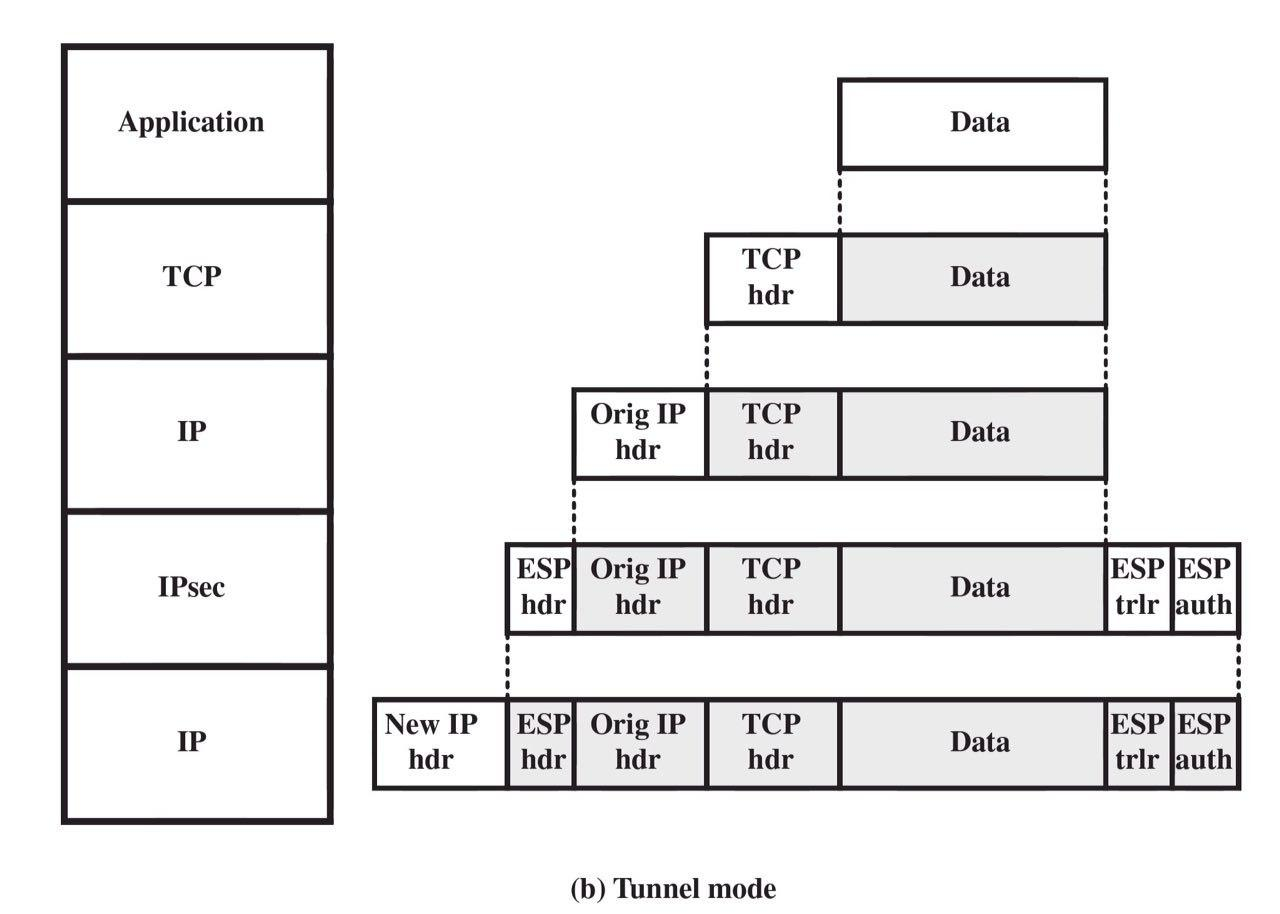
\includegraphics[scale=0.20]{ESPauthTun.jpg}
  \end{itemize}
}
  

\frame{\frametitle{Transport Adjacency}
  Se utilizan dos \textit{SAs} de transporte agrupadas, la primera o interior
  consta de aplicar \textit{ESP} sin autentificación, la segunda o exterior, consta de aplicar \textit{AH}
  en modo de transporte para que pueda cubrir tanto la parte del \textit{ESP} y la cabecera original del paquete.
}

\frame{\frametitle{Transport-Tunnel Bundle}
  En este caso se utiliza primero autentificación y posteriormente cifrado.
  Se aplica la asociación de seguridad \textit{AH} sobre la carga útil del paquete \textit{IP} junto con su cabecera. El paquete resultante
  se procesa con una segunda asociación de seguridad \textit{ESP} con modo de túnel. Al ser aplicado sobre todo el paquete, debe agregarse
  una nueva cabecera \textit{IP}.
}


\subsection{Combinaciones básicas}
\frame{\frametitle{Combinaciones básicas de SAs}
  \textbf{Caso 1.}
  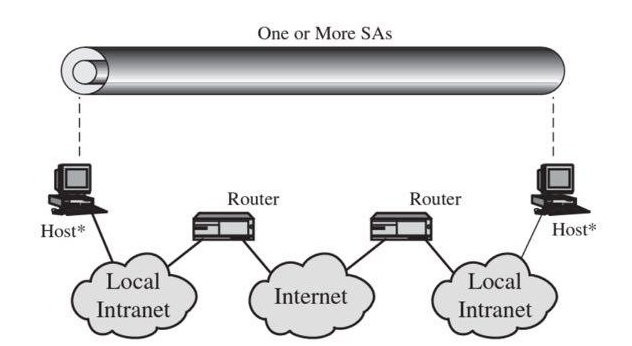
\includegraphics[scale=0.45]{caso1}
}

\frame{\frametitle{Combinaciones básicas de SAs}
  \textbf{Caso 2.}
  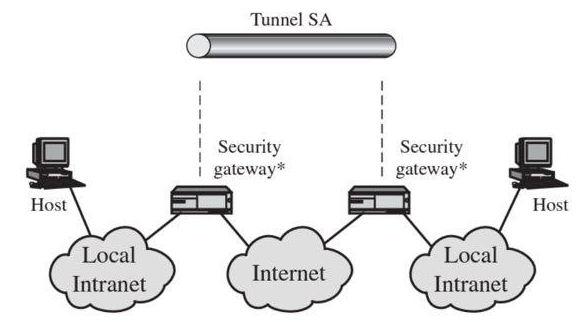
\includegraphics[scale=0.47]{caso2}
}

\frame{\frametitle{Combinaciones básicas de SAs}
  \textbf{Caso 3.}
  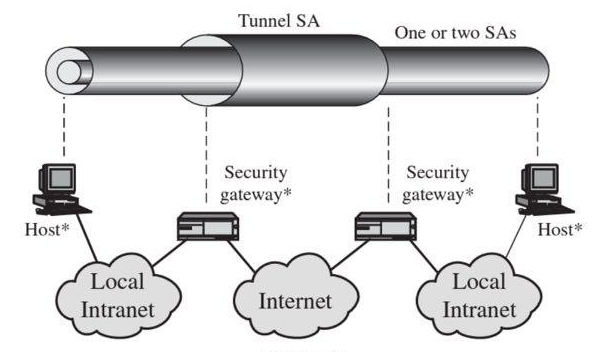
\includegraphics[scale=0.45]{caso3}
}

\frame{\frametitle{Combinaciones básicas de SAs}
  \textbf{Caso 4.}\\
  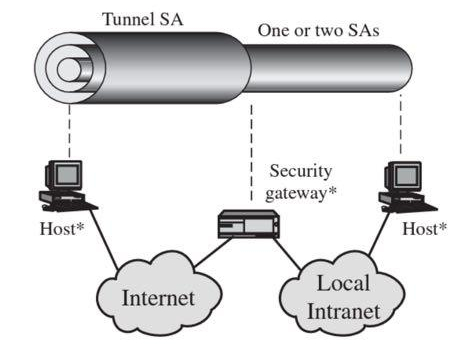
\includegraphics[scale=0.45]{caso4}
}


\section{Internet Key Exchange (IKE)} 
\subsection{Definición}
\frame{\frametitle{Internet Key Exchange (IKE)}
  Determinación y distribución de llaves secretas. Típicamente se requiere de cuatro llaves, dos pares para transmisión y recepción (para integridad y confidencialidad). \\~\\

  Tipos de manejo de llaves:
  \begin{itemize}
  \item \textbf{Manual:} Un administrador configura cada sistema con sus propias llaves y las de otros sistemas.
  \item \textbf{Automatizado:} Un sistema automatizado permite la creación de llaves para las asociaciones de seguridad.
  \end{itemize}
}

\frame{\frametitle{ISAKMP/Oakley}
  Protocolo por defecto de manejamiento de llaves automatizado. Consiste en: \\
  \begin{itemize}
  \item \textbf{Protocolo de determinación de llaves Oakley}: Protocolo de intercambio de llaves basado en el algoritmo Diffie-Hellman con seguridad agregada.
  \item \textbf{Asociación de seguridad de Internet y Protocolo de Manejo de Llaves (ISAKMP)}: ISAKMP provee un framework para el manejo de llaves por internet.
  \end{itemize}  
}

\subsection{Protocolo de determinación de llaves}
\frame{\frametitle{Protocolo de determinación de llaves}
  Refinamiento del intercambio de llaves Diffie-Hellman: \\~\\
  
  A y B se ponen de acuerdo en $q$ y $\alpha$ (raíz primitiva). \\  
  A selecciona $X_A$, B selecciona $X_B$ \\
  A calcula $Y_A \equiv \alpha^{X_A} \Mod{q}$, B calcula $Y_B \equiv \alpha^{X_B} \Mod{q}$ \\
  A y B calculan la llave secreta $K$: \\
  $K \equiv (Y_B)^{X_A} \Mod{q} \equiv (Y_A)^{X_B} \Mod{q} \equiv \alpha^{X_AX_B} \Mod q$
}

\frame{\frametitle{Protocolo de determinación de llaves}
  Beneficios de Diffie-Hellman: \\~\\
  
  \begin{itemize}
  \item Las llaves se crean cuando se necesitan.
  \item Sólo de necesita ponerse de acuerdo en los parámetros globales.
  \end{itemize}  
}

\frame{\frametitle{Protocolo de determinación de llaves}
  Debilidades de Diffie-Hellman: \\~\\
  
  \begin{itemize}
  \item No provee información sobre los participantes.
  \item Susceptible al ataque $man$-$in$-$the$-$middle$.
  \item Es intenso computacionalmente, lo que lo hace vulnerable a ataques de $clogging$.
  \end{itemize}
}

\subsubsection{Propiedades de IKE}

\frame{\frametitle{Propiedades de IKE}
  \begin{itemize}
  \item Utiliza cookies para evitar ataques de $clogging$.
  \item Permite negociar los parámetros globales.
  \item Utiliza $nonces$ para evitar ataques de repetición.
  \item Permite que se lleve acabo el intercambio de llaves públicas de Diffie-Helman.
  \item Autentifica para evitar ataques $man$-$in$-$the$-$middle$.
  \end{itemize}
}

\frame{\frametitle{Cookies}
  \textbf{Problema}: Oponente se hace pasar por una fuente legítima y manda repetidamente llaves públicad de Diffie-Hellman a la víctima. \\~\\

  \textbf{Solución}: Intercambio de $cookies$. Cada lado manda un número aleatorio ($cookie$) que es reconocido por el otro lado. Este reconocimiento se repite en el primer mensaje del intercabio Diffie-Hellman.
}

\frame{\frametitle{Cookies}
  Carácterísticas del cookie: \\~\\

  \begin{itemize}
  \item Depende de los lados que se comunican.
  \item No debe ser posible, más que para la entidad que le concierne, generar cookies que serán aceptadas por dicha entidad. Se usa información local secreta en el uso y verificación del cookie.
  \item La generación y verificación de cookies debe ser rápida.
  \end{itemize}
}

\frame{\frametitle{Grupos para D-H}
  Exponenciación modular con módulo de 768 bits \\
  $q = 2^{768} - 2^{704} - 1 + 2^{64} \times (\floor{2^{638} \times \pi} + 149686)$ \\
  $\alpha = 2$ \\~\\

  Exponenciación modular con módulo de 1024 bits \\
  $q = 2^{1024} - 2^{960} - 1 + 2^{64} \times (\floor{2^{864} \times \pi} + 129093)$ \\
  $\alpha = 2$ \\~\\

  Exponenciación modular con módulo de 1536 bits.
  
}

\frame{\frametitle{Grupos para D-H}
  Curva elíptica sobre $2^{155}$ \\
  Generador: (7B, 1C8) \\
  Parámetros: A = 0, B = 1EE9 \\~\\

  Curva elíptica sobre $2^{185}$ \\
  Generador: (18, D) \\
  Parámetros: A = 0, B = 1EE9
}

\frame{\frametitle{Métodos de Autenticación}
  \begin{itemize}
  \item \textbf{Firmas digitales}: Se firma un hash por ambos lados, cada uno con su propia llave privada. El hash se genera con el ID de usuario y $nonces$.
  \item \textbf{Cifrado de llave publica}: Se cifran parámetros como IDs y $nonces$ con la llave privada del remitente.
  \item \textbf{Cifrado con llave simétrica}: Se usa un sistema de cifrado simétrico.
  \end{itemize} 
}

\subsubsection{IKEv2}
\frame{\frametitle{}
  
}

\subsection{Formatos de encabezado y payload}
\subsubsection{Formato del encabezado IKE}
\subsubsection{Tipos del payload IKE}
\frame{\frametitle{}
  
}
\section{Suites criptográficas}
\subsection{}
\frame{\frametitle{}
}
\end{document}

